Přihlašování uživatelů probíhá identickým způsobem pro Frontend i Backend. Aplikace je dostupná pouze pro přihlášené, pokus o přístup bez platného přihlášení vyvolá přesměrování na SignPresenter. Přestože základní URL adresa aplikace vede na \texttt{Homepage:default}, (nepřihlášení) uživatelé jsou vždy přesměrováni nejdříve na~přihlašovací stránku.

\begin{figure}[h]
	\centering
	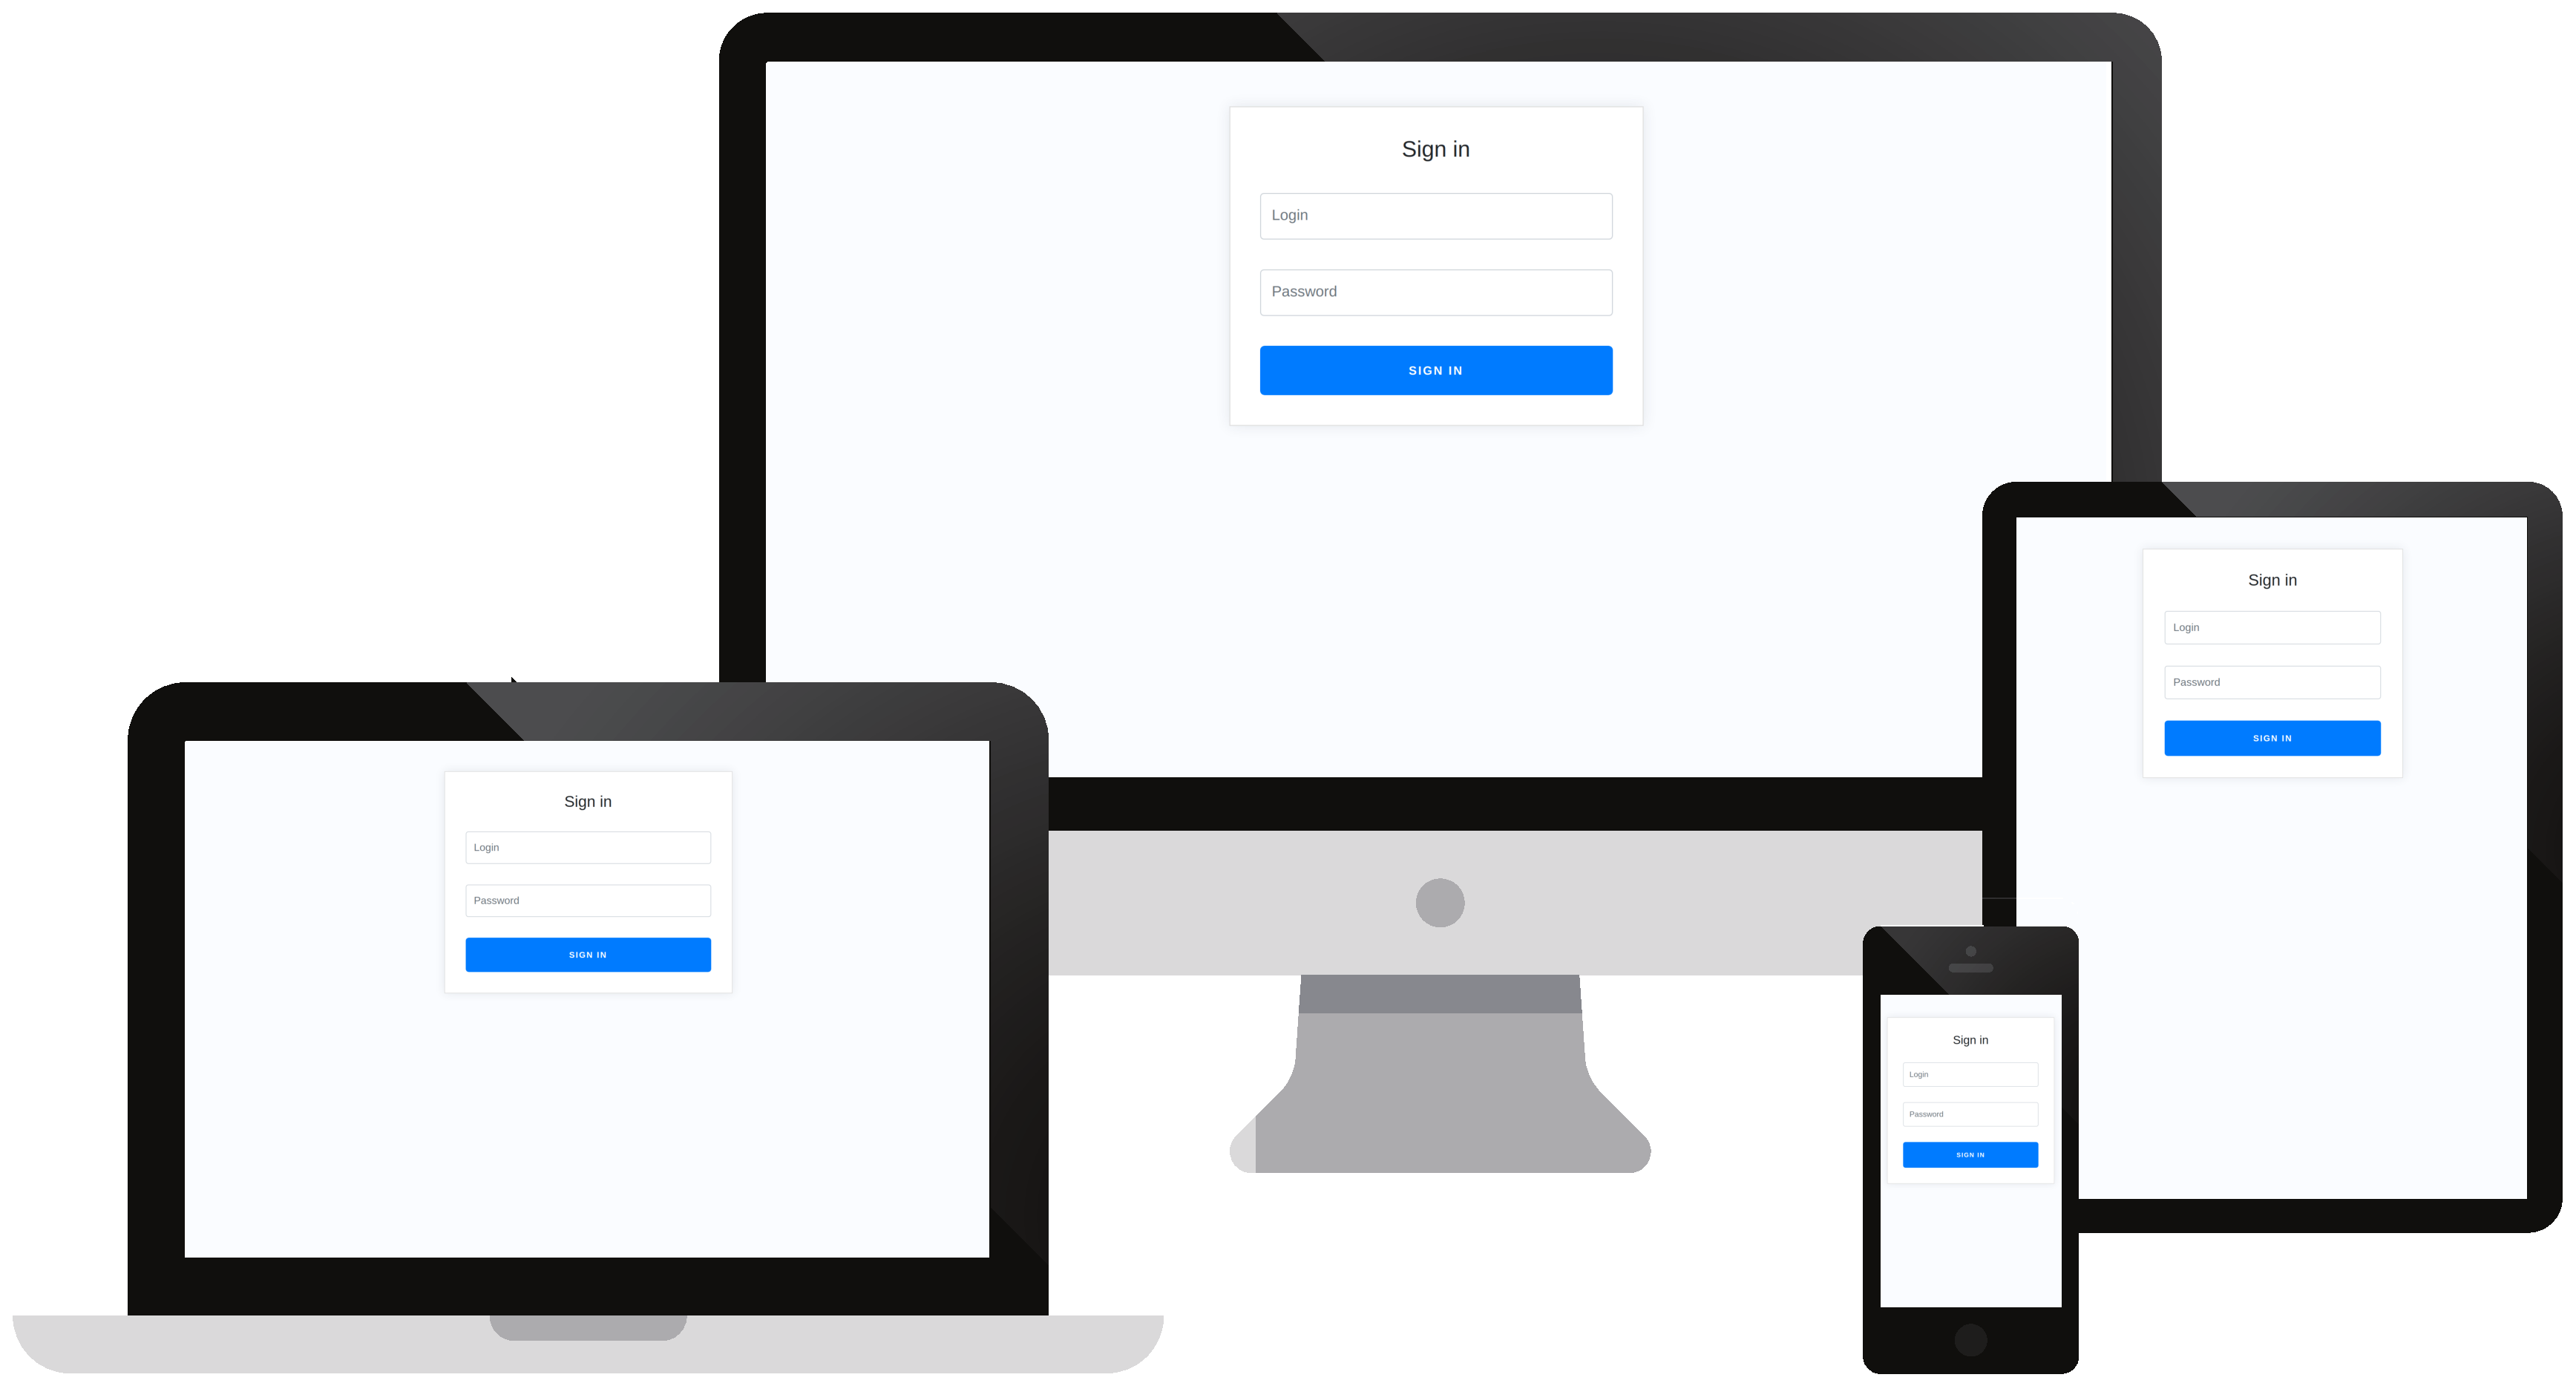
\includegraphics[width=\linewidth]{svg/mockup/prihlasovani.eps}
	\captionsetup{width=\linewidth}
	\caption[Vzhled přihlašovacího formuláře]{Vzhled přihlašovacího formuláře (zdroj: vlastní, Freepik.com)}
	\label{mockup:login}
\end{figure}

K ověření (autentizaci) uživatele pomocí kombinace uživatelského jména (e-mailové adresy) a hesla v Nette slouží rozhraní \texttt{Authenticator}\footnote{\Verb{Nette\Security\Authenticator}}. Samotný proces ověření inicializuje objekt \texttt{User}\footnote{\label{user}\Verb{Nette\Security\User}}. 

SignPresenter po odeslání formuláře předá objektu \texttt{User} implementaci rozhraní a následně zavolá metodu \phpinline{User::login($username, $password)}. Pokud ověření selže, je vyvolána výjimka \texttt{AuthenticationException}, která je zachycena v presenteru. Úspěšná autentizace způsobí uložení implementace \texttt{IIdentity} do objektu \texttt{User}.

Jedním z požadavků na aplikaci byla stanovena možnost přihlášení voličů pomocí univerzitních e-mailových adres. Implementace ověřování metodou Single Sign-On přes systém Shibboleth by byla nad rámec této práce a po diskuzi s vedoucím práce bylo zvoleno ověřování pomocí Active Directory přes LDAP. Dalším požadavkem byla možnost přihlášení externích uživatelů bez nutnosti vytvářet jim univerzitní e-mailové adresy. Tohoto bylo docíleno možností ověření vůči databázi aplikace.
\clearpage
\begin{listing}[ht]
\phpsnippet{tex/code/autentizace.php}
\caption{Autentizace v SignPresenter}
\label{php:autentizace}
\end{listing}

K autentizaci se využívají dvě implementace třídy \texttt{Authenticator}. První se k~ověření použije \texttt{PasswordAuthenticator}, která při úspěšném ověření vrací entitu uživatele včetně všech rolí, při neúspěchu následuje pokus o ověření přes \texttt{LdapAuthenticator}.

\begin{itemize}
	\item \textbf{PasswordAuthenticator} - v prvním kroku získá na základě e-mailové adresy entitu uživatele z repozitáře. Pokud takový uživatel v databázi není, je vyvolána výjimka \texttt{AuthenticationException}. V druhém kroku předá uloženou hash hesla a ověřované heslo třídě \phpinline{Nette\Security\Passwords} k porovnání. Pokud heslo neodpovídá, je opět vyvolána výjimka. Úspěšné ověření vrátí získanou entitu.
	\item \textbf{LdapAuthenticator} - v prvním kroku se pokusí ověřit kombinaci e-mailové adresy a hesla vůči univerzitnímu Active Directory, při neúspěchu vyvolá výjimku. V druhém kroku se pokusí získat z repozitáře entitu uživatele s~odpovídající \mbox{e-mailovou} adresou, pokud takový neexistuje, je vytvořena nová entita s rolemi získanými z Active Directory. Tyto role jsou buď \textit{Student} nebo \textit{Zaměstnanec}.
\end{itemize}

